\section{Anhang}
\label{sec:anhang}

		\begin{figure}[H]
		    \centering
				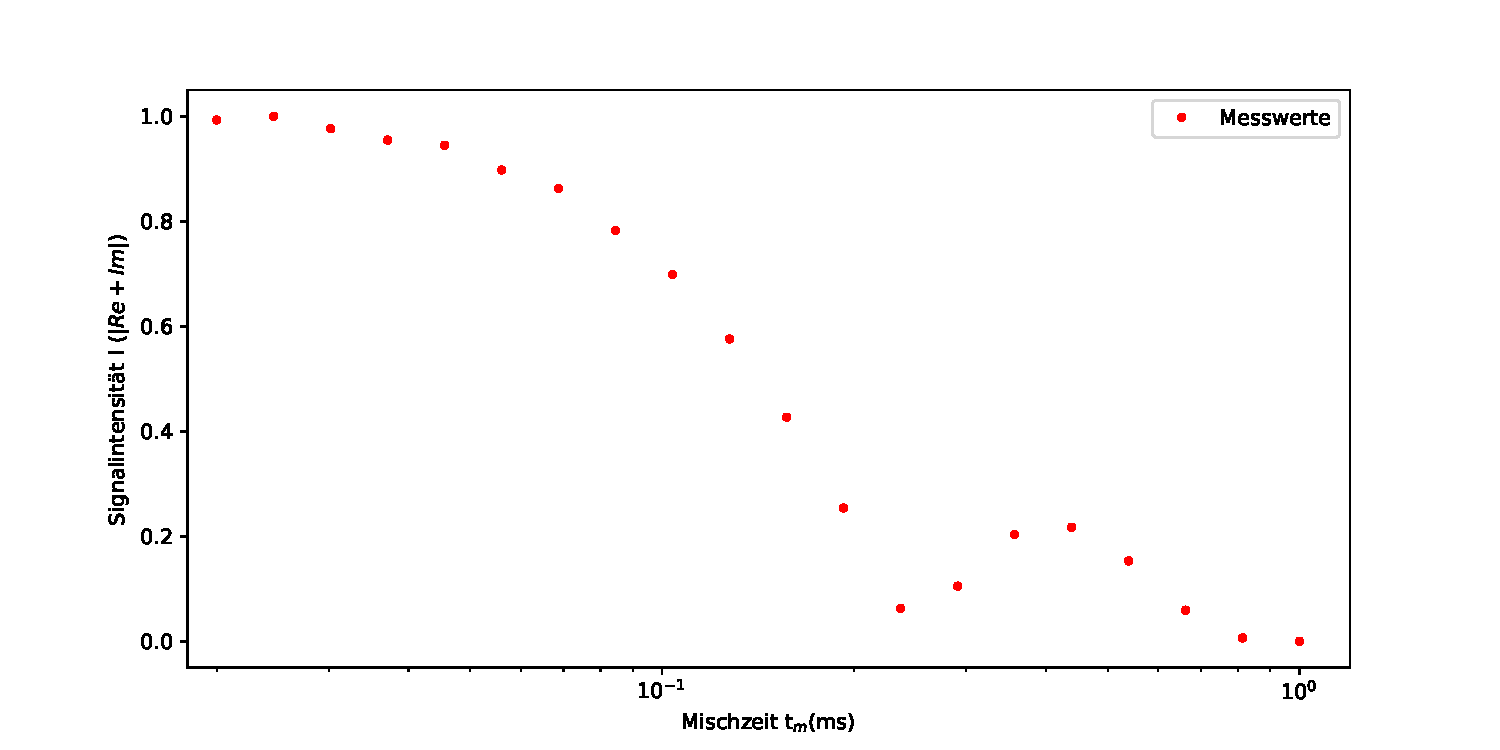
\includegraphics[width=\textwidth]{Auswertung/Tempabh/Abb/T2/DMSO2_T2_319K.dat.nmr.pdf}
		    \caption{$T_2$-Messung bei $\SI{319}{\kelvin}$. Besonders auffällig ist der plötzliche
				Anstieg des Mess-Signals bei etwa $\SI{0,2}{\milli\second}$, welche das anlegen
				der Kohlrauschfunktion nicht möglich macht.}
		    \label{fig:T2err}
		\end{figure}
		\noindent
